% Periodic boundaries conditions
% Germain Salvato-Vallverdu - may 2009
% http://germain.salvato-vallverdu.perso.sfr.fr
\documentclass[11pt,a3paper,landscape]{article}

\usepackage[utf8]{inputenc}
\usepackage{graphicx}

\usepackage{tikz}

%\usepackage{standalone}

%%%<
\usepackage{verbatim}
%\usepackage[active,tightpage]{preview}
%\PreviewEnvironment{tikzpicture}
%\setlength\PreviewBorder{5pt}%
%%%>

\begin{comment}
:Title: Periodic boundaries conditions
:Zip: img/wat.png, img/wat3.png, img/wat2.png, img/wat4.png

In condensed matter simulation periodic boundaries conditions are
often used to simulate an infinite system.

\end{comment}

\title{Periodic boundaries conditions}
\author{Germain Salvato-Vallverdu}

\usepackage{hyperref}
\hypersetup{%
pdfauthor={Germain Salvato-Vallverdu},%
pdftitle={Periodic boundaries conditions},% 
pdfkeywords={Tikz,latex,Periodic boundaries conditions,simulation},%
pdfcreator={PDFLaTeX},%
pdfproducer={PDFLaTeX},%
}

\pagestyle{empty}

\begin{document}
\begin{center}

\begin{tikzpicture}

% water molecule in the initial simulation box
\path (0.45,3.3) node {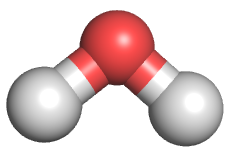
\includegraphics[width=0.75cm]{img/wat}}
      (1.6,4.4)  node {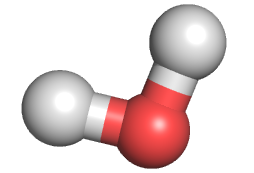
\includegraphics[width=0.75cm]{img/wat3}}
      (0.5,4.45) node {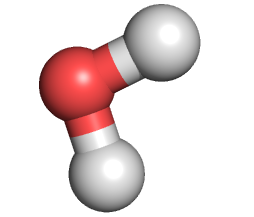
\includegraphics[width=0.75cm]{img/wat2}}
      (1.1,3.7)  node {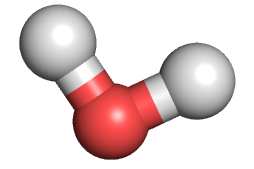
\includegraphics[width=0.75cm]{img/wat4}};

% edge of the initial simulation box
\path[draw,ultra thick] (0,3) rectangle (2,5);

% periodic boundaries
\foreach \x in {5,7,9} {
    \foreach \y in {1,3,5} {
        % water molecules in images
        \node at (\x+0.45,\y+0.3) {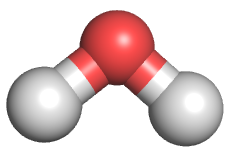
\includegraphics[width=0.75cm]{img/wat}};
        \node at (\x+1.6 ,\y+1.4) {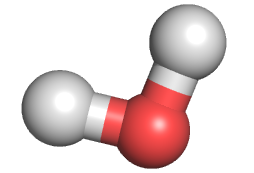
\includegraphics[width=0.75cm]{img/wat3}};
        \node at (\x+0.5 ,\y+1.45) {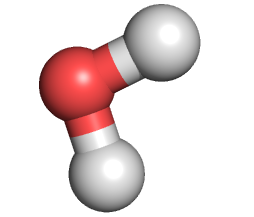
\includegraphics[width=0.75cm]{img/wat2}};
        \node at (\x+1.1 ,\y+0.7) {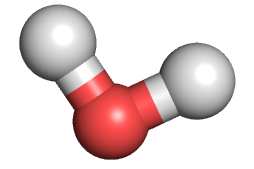
\includegraphics[width=0.75cm]{img/wat4}};
        
        % edge of each box
        \path[draw,thick] (\x,\y) rectangle (\x+2,\y+2);
    }
}

% central box thicker than other
\path[draw,ultra thick] (7,3) rectangle (9,5);

% an arrow
\path[draw,ultra thick,->] (2.5,4) -- (4.5,4);

% dashed lines 
\foreach \x in {5,7,9,11} {
    % vertical
    \path[draw,dashed,thick] (\x,0) -- (\x,1) (\x,7) -- (\x,8);
    % horizontal
    \path[draw,dashed,thick] (4,\x-4) -- (5,\x-4) (11,\x-4) -- (12,\x-4);
}

\end{tikzpicture}

\end{center}

\end{document}